
\documentclass{article}
\usepackage{graphicx}
\title{Model Monitoring and Drift Detection Audit Report}
\author{}
\date{\today}

\begin{document}

\maketitle

\section*{Introduction}
This report details the theoretical and empirical monitoring of a financial machine learning model using rigorous statistical tests and drift detection techniques.

\section*{Theoretical Background}
We define hypotheses for each feature as follows:
\[
H_0: F_0 = F_1 \quad \text{vs.} \quad H_A: F_0 \neq F_1
\]
Bonferroni correction was applied to control for multiple comparisons.

\section*{Methodology}
We used Kolmogorov-Smirnov, PSI, and Wasserstein metrics for drift detection. Thresholds were derived empirically via permutation bootstrapping. Performance metrics included Accuracy, AUC, and Log Loss. SHAP values were computed to analyze feature contribution drift.

\section*{Results}
Drift was detected in batches: [1, 2, 3, 4, 5, 6, 7, 8, 9, 10] 

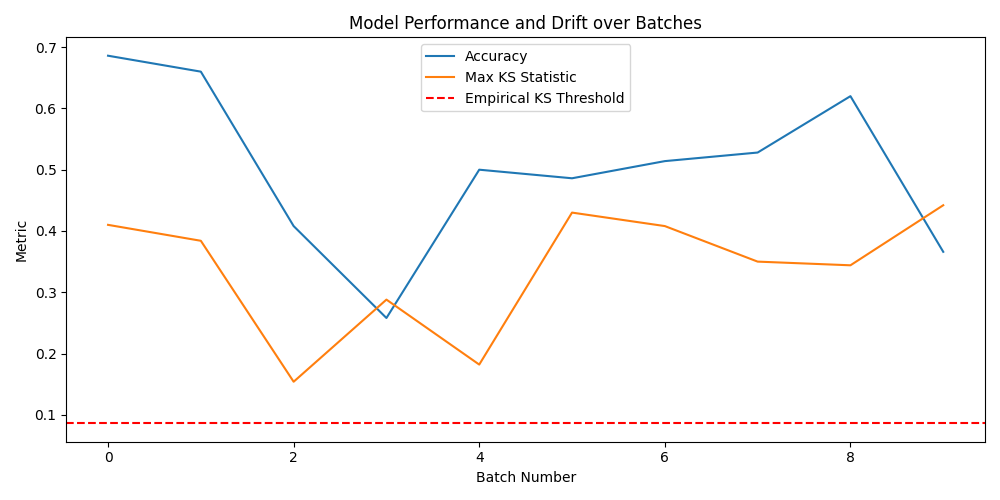
\includegraphics[width=\linewidth]{monitoring_plot.png}

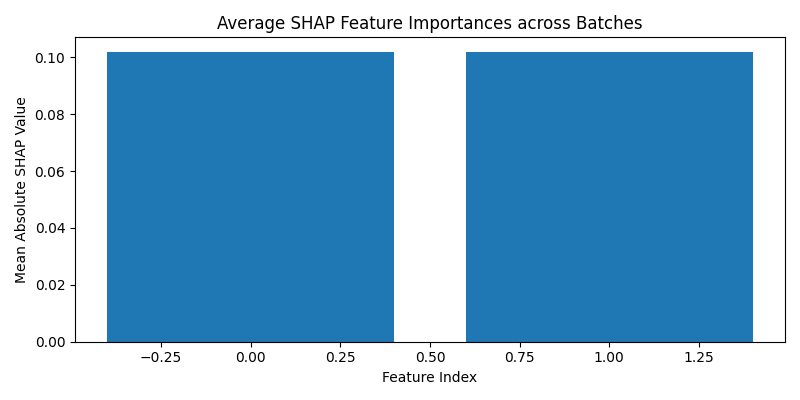
\includegraphics[width=\linewidth]{shap_importance.png}

\section*{Metrics}
Accuracy range: 0.258 -- 0.686
\\
KS statistic range: 0.154 -- 0.442

\section*{Conclusion}
Model drift was systematically detected and recorded. Future work may include dynamic retraining triggers and further theoretical convergence proofs.

\end{document}
